\subsubsection{Pourquoi JavaFX ?}

Une question que nous nous sommes posée est : Swing ou JavaFX ?

Nous avons choisi d'utiliser JavaFX pour une principale raison. JavaFX est désormais la librairie officielle de Java. Swing n'étant plus maintenu, nous ne voulions pas développer avec une librairie qui commence à être dépréciée.

De plus, le sujet de Bataille Navale (le projet de Complément de POO que nous devons réaliser en parallèle) étant à faire obligatoirement en swing, nous voulions essayer les deux librairies.


\subsubsection{L'interface graphique}

Le développement de l'interface graphique a progressé au rythme du reste du projet, implémentant ce qui a été codé en parallèle. Plusieurs optimisations ont cependant été réalisées pour que l'affichage à l'écran impacte le moins possible les performances générales.

L'optimisation la plus impactant est l'usage d'un IntBuffer et de PixelFormat<IntBuffer>. Ils ont permis d'utiliser la méthode setPixels de PixelWriter, permettant ainsi de définir les pixel de la fenêtre de rendu d'un coup et non pas pixel par pixel comme fait précédememnt.

Un des effets secondaires engendrés par les calculs lourds du rendu est la fenêtre qui n'était plus réactive.
Au départ, nous utilisions CameraTimer et WindowTimer, deux classes héritant de Animation Timer. WindowTimer lançait le rendu et CameraTimer s'occupait de gérer un déplacement de caméra. La méthode handle de AnimationTimer s'exécute à chaque frame, ce qui nous permettait de gérer l'affichage des FPS, la caméra et le rendu à l'aide de la méthode handle et tout était donc synchronisé.

Le problème posé par ce choix était que JavaFX gérait directement les calculs de rendus. La conséquence était une interface graphique réactive à la vitesse du rendu (quelques images par seconde).

\label{UsageTask}

Pour palier à ce problème, nous avons utilisé des classes proposées par le package concurrent de JavaFX. Le problème a été résolu grâce à la classe tasks de ce package, permettant de faire des calculs lourds sans impacter la réactivité de l'interface graphique. Comme javafx et le calcul de rendu n'étaient plus liés il a fallu synchroniser les mouvements de caméra et le calcul de l'image d'après.

\subsubsection{La Toolbox}

La toolbox est un élément essentiel du raytracing. Elle permet à l'utilisateur d'utiliser le logiciel avec simplicité, sans devoir passer par des lignes de commandes ou des scripts d'exécution.
Ensuite, le logiciel de rendu utilise différents procédés qui peuvent fonctionner en parallèle ou les uns au-dessus des autres. La toolbox permet de choisir quels éléments l'utilisateur veux conserver pour pouvoir ainsi mieux comprendre les différentes étapes jusqu'au rendu final.
Pour finir, cette interface permet à l'utilisateur d'avoir un maximum de liberté sur l'utilisation du logiciel, lui permettant ainsi de faire un compromis entre fidélité et rapidité.

\begin{figure}[h]
   \begin{center}
       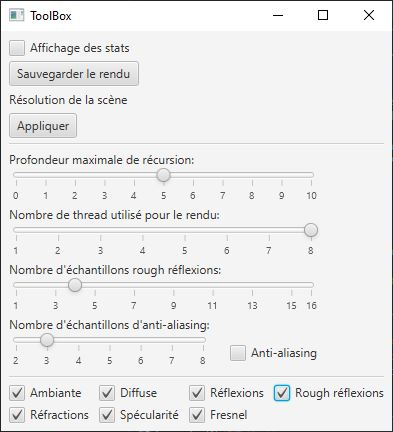
\includegraphics[scale=0.8]{img/rt/toolbox.jpg}
   \end{center}
   \caption{La toolbox et les possibilités qu'elle offre.}
\end{figure}
\FloatBarrier



\subsubsection{Le CSS}

En quelques mots, JavaFX permet de lier le style de ces fenêtres à des fichiers CSS. Nous en avons profité pour aérer les fenêtres de choix de taille et la "toolbox".

\subsubsection{Le mode automatique}

Le mode automatique récupère la taille de l'écran principal, maximise la fenêtre et étire le rendu de manière à ce qu'il soit pixélisé, mais qu'il occupe tout l'écran.

Dans une version plus ancienne, la taille du rendu était également fixée par la taille de la fenêtre. Suite à l'ajout de la réfraction et de l'uvsphère qui sont assez coûteuses en ressource nous avons décidé de supprimer cette fonctionnalité.

\subsubsection{Le conteur de fps}

Le conteur de FPS tire parti des avantages offerts par la classe AnimationTimer et utilise l'horodatage fournit par celle-ci pour calculer la vitesse de rendue.
